\section{Class-I and Class-II: structure with and without drive}
\label{sec:class-i-ii}

Class-I and Class-II both form structure, so both have packaging switched on. They differ in one respect only: whether directed circulation is present when the structure forms. This is the cleanest contrast in the paper.

\paragraph{Representatives.} The Class-I representative is a reversible two-block kernel. It has $N=32$ states in two blocks of 16, uniform within-block weight $1$, and cross-block weight $0.25$. The kernel is symmetric. The Class-II representative is a biased ring on $N=32$ states with stay, forward, and backward weights $0.10$, $0.55$, and $0.35$. Both are analysed with the manual two-block lens. Table~\ref{tab:class-i-ii-summary} gives their readings, which coincide with the exact certificates of Table~\ref{tab:certificates}.

\begin{table}[tbp]
\centering
\small
\caption{Class-I and Class-II reference readings ($N=32$, manual lens, $\tau=1$). The asterisk marks a left-censored boundary. Affinity is the floating-point reading at $\lambda_{\mathrm{struct,ref}}$; the exact lower bound is in parentheses.}
\label{tab:class-i-ii-summary}
\setlength{\tabcolsep}{4pt}
\begin{tabular}{@{}lccccccc@{}}
\toprule
Class & $\lambda_{\mathrm{CE}}$ & $\lambda_{M_{\mathrm{obj}}}$ & $\lambda_{\mathrm{struct,ref}}$ & $\mathrm{Aff}_{\mathrm{ref}}$ & $\Delta\lambda_{\mathrm{CE}}$ & $\Delta\lambda_{M_{\mathrm{obj}}}$ & Label \\
\midrule
I  & 0.874 & 0.763 & 0.874 & $0$ (exact) & 0.062 & 0.115 & Class-I \\
II & 0.556 & 0.500$^{*}$ & 0.556 & $3.45\times10^{-2}$ ($\ge 3.40\times10^{-2}$) & 0.189 & 0.000 & Class-II \\
\bottomrule
\end{tabular}
\end{table}

\paragraph{Both form structure.} Each representative reaches CE${}\le0.025$ and $M_{\mathrm{obj}}\ge0.90$ on its grid, so packaging is on for both (Figure~\ref{fig:structural-curves}, first two columns). Class-II forms structure at smaller closure strength. Its objecthood threshold is already met at the first grid point, $\lambda=0.5$, so only an upper bound is known for $\lambda_{M_{\mathrm{obj}}}$. This does not affect the label, because the closure boundary at $0.556$ is resolved and is the larger of the two.

\begin{figure}[tbp]
\centering
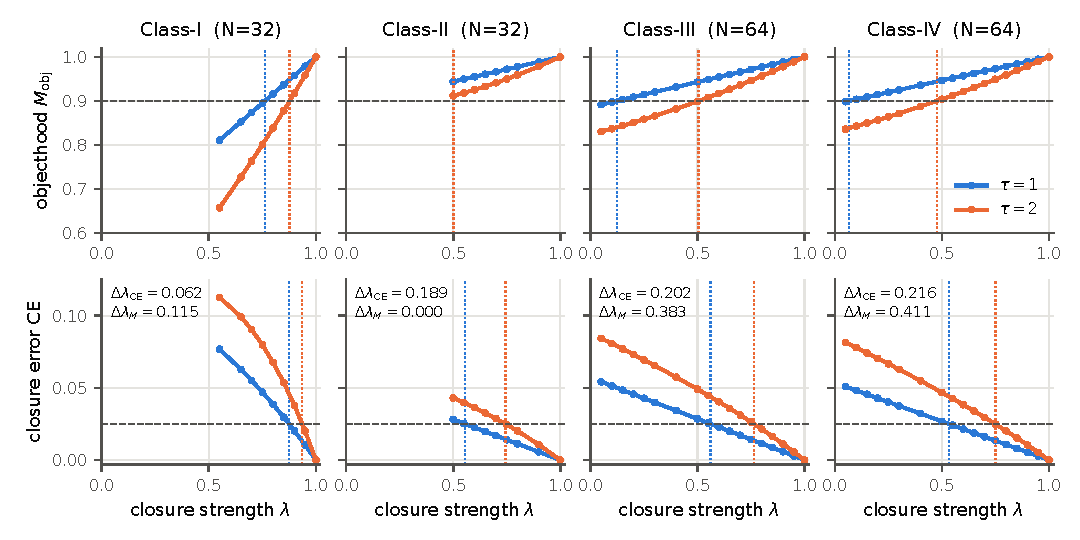
\includegraphics[width=\textwidth]{figures/structural_curves.pdf}
\caption{Exact structural curves of the four representatives (manual lens), at $\tau=1$ (blue) and $\tau=2$ (orange). Top row: objecthood, with threshold $0.90$. Bottom row: closure error, with threshold $0.025$. Dotted verticals mark the boundaries; the shifts between the two timescales are printed in each lower panel. Class-I and Class-II each have at least one small shift, so staging is off. Class-III and Class-IV have both shifts above $0.15$, so staging is on. Curve values are exact rationals at the grid points.}
\label{fig:structural-curves}
\end{figure}

\paragraph{Only Class-II carries drive.} The Class-I kernel and its mixtures with $QU$ are symmetric, so by Proposition~\ref{prop:reversal} the affinity is exactly zero at every $\lambda$. Class-II has $\mathrm{Aff}_{\mathrm{ref}}=3.45\times10^{-2}$ at its structural boundary. The exact lower bound, $3.40\times10^{-2}$, is more than an order of magnitude above the drive-on threshold of $10^{-3}$. Figure~\ref{fig:drive-curves} shows the affinity along the closure-strength axis. For Class-II it stays above $10^{-2}$ from $\lambda=0.5$ to $0.8$ and falls to zero at $\lambda=1$, where the dynamics becomes the symmetric kernel $QU$. Because the Class-I value is exactly zero, a ratio between the two affinities is meaningless. The relevant fact is the absolute gap: zero against a value well inside the drive-on region.

\begin{figure}[tbp]
\centering
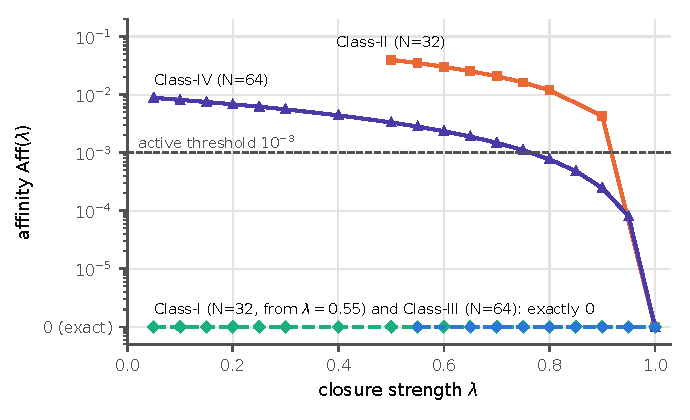
\includegraphics[width=0.66\textwidth]{figures/drive_curves.pdf}
\caption{Affinity along the closure-strength axis for the four representatives (manual lens, $\tau=1$). Class-I and Class-III are exactly zero on their whole grids (plotted on the floor). Class-II and Class-IV are positive until $\lambda=1$, where packaging replaces the dynamics by the symmetric kernel $QU$. The dashed line is the drive-on threshold.}
\label{fig:drive-curves}
\end{figure}

\paragraph{Staging is detectable but off.} Both representatives show some sensitivity to the timescale, so both have a $P4$-like signal (Table~\ref{tab:rubric}). Neither meets the strict rule. In Class-I both boundaries move, but by less than $0.15$ ($0.062$ and $0.115$). In Class-II the closure boundary moves by $0.189$ while the objecthood boundary does not move at all. This is exactly the case the two-level staging rule is designed for: a timescale effect that shows up in one channel only is recorded, but it does not make the birth a staging birth.

\paragraph{Controls against false arrows.} A drive axis is useful only if reversible systems are not mislabelled as driven. We ran two kinds of control (Table~\ref{tab:no-fake-arrow-summary}):
\begin{itemize}
  \item \emph{Reversible controls.} These are a reversible block kernel under the manual lens, the same kernel under the spectral lens, and a flat-mixing null kernel. All three have zero affinity and are not flagged as driven.
  \item \emph{Protocol-trap controls} \cite{sixbirds_protocol_trap}. Three reversible phase kernels are applied in a fixed cyclic order. When the ordered product is read as a single time-homogeneous kernel (the \emph{hidden-schedule} reading), it has affinity $0.058$ and is flagged as a driven candidate. Each constituent phase kernel, examined on its own (the \emph{phase-resolved} reading), has zero affinity and is not flagged.
\end{itemize}
The reversible controls show that the drive channel does not produce arrows out of reversible dynamics. The protocol trap shows that the channel reports on the kernel it is given: hiding the schedule produces an effective kernel that is genuinely non-reversible. This control does not construct the full autonomous process with an explicit phase register, so it is not a theorem that phase-aware handling always removes the arrow. Its purpose is narrower: to check that the audit separates the two readings as intended.

\begin{table}[tbp]
\centering
\small
\caption{No-fake-arrow controls.}
\label{tab:no-fake-arrow-summary}
\setlength{\tabcolsep}{4pt}
\begin{tabularx}{\linewidth}{@{}Y l l@{}}
\toprule
Control & Affinity & Flagged as driven? \\
\midrule
Protocol trap, hidden schedule (ordered product as one kernel) & 0.0576 & yes \\
Protocol trap, phase-resolved (each of the three phase kernels) & 0 & no \\
Reversible block kernel, manual lens & 0 & no \\
Reversible block kernel, spectral lens & 0 & no \\
Flat-mixing null kernel & 0 & no \\
\bottomrule
\end{tabularx}
\end{table}

\paragraph{Robustness.} Two further checks support the contrast. First, small-size robustness runs ($n=8$) swapped the manual lens for the spectral or the diffusion lens. For the reversible family the sampled birth window stayed at $[0.75,1]$. For the driven family it moved by one sampled interval, from $[0.5,0.75]$ to $[0.75,1]$, which is within the configured stability tolerance of one grid interval. This checks the approximate location of the structural window under a lens swap; it is not a full re-classification under those lenses. Second, in a scan over drive bias the affinity grows monotonically with the bias, while the structural boundary under the baseline $\tau=1$ analysis does not move. At $\tau=2$, however, some coupling between bias and structure is visible. In this sense drive behaves as a separate channel from packaging, but the separation is a property of the declared scan and is not proved in general.

\paragraph{Summary.} Class-I and Class-II are two distinct birth classes with the same structural switch and opposite drive switches. The difference is carried by an exact zero against a certified positive affinity, and the controls show that the drive channel does not invent arrows. This result needs no exponent fit, and it is the most robust result in the paper.
